\documentclass[11pt,a4paper]{article}
\usepackage[margin=2.2cm]{geometry}
\usepackage{graphicx}
\usepackage{booktabs}
\usepackage{longtable}
\usepackage{array}
\usepackage{xcolor}
\usepackage[expansion=false]{microtype}
\usepackage[hidelinks]{hyperref}

\definecolor{accent}{RGB}{140,60,20}
\newcommand{\net}[1]{\texttt{#1}}

\title{\textbf{pd-trigger} --- USB-C Power Delivery Trigger Board\\
\large Design Document, rev.\ v1 (S14 run~c)}
\author{ai-ee pipeline --- AI-generated design, human-reviewed gates}
\date{28 July 2026}

\begin{document}
\maketitle

\begin{abstract}
\noindent A bench USB-C Power Delivery \emph{sink} trigger: negotiates a
user-selected PD profile (5/9/12/15/20\,V) from any PD source and delivers
it on a screw terminal, sized for 5\,A continuous (100\,W at 20\,V).
CH224K sink controller, DIP-switch profile straps, zener-window fallback
indication, 48$\times$30\,mm, 2-layer \textbf{2\,oz} copper, JLCPCB economy
assembly. All five machine gates green (ERC, placement, routed DRC,
8-check verification, gerber DFM); two adversarial design reviews passed.
Estimated \$19.65 for 10 assembled (quote-page price is authoritative).
\end{abstract}

\section{Requirements}
\begin{itemize}\itemsep2pt
  \item USB-C receptacle, PD \textbf{sink} only --- no USB data. ``PD SRC
        ONLY'' is printed at the connector: legacy QC/BC adapters supply
        5\,V fallback only (by design, see \S\ref{sec:decisions}).
  \item Output profiles 5/9/12/15/20\,V, selected on-board; uniform
        \textbf{5\,A} rating at every profile; screw terminal
        ($\geq$8\,A, 18\,AWG) plus a low-current auxiliary header
        (``AUX 1A MAX'' silk).
  \item Fallback to 5\,V when the source cannot deliver the selected
        profile is acceptable but must be \emph{visibly indicated}.
  \item Bench use, no enclosure, no battery; prototype qty 10; JLC Basic
        parts preferred; soft size target $\sim$40$\times$25\,mm (+20\%
        allowance used: final 48$\times$30\,mm).
\end{itemize}

\section{Architecture}
Signal/power chain:
\begin{center}
\small
\net{J1 USB-C} $\rightarrow$ \net{VBUS} pour fan-in $\rightarrow$
TVS \net{D1} + bulk \net{C1A/C1B/C2} $\rightarrow$
\textbf{3.0\,mm trunk} $\rightarrow$ \net{J2 screw terminal}\\[2pt]
taps: \net{R14 0R} $\rightarrow$ \net{/VIND} housekeeping;\quad
\net{F1 PPTC 1A} $\rightarrow$ \net{/VAUX} $\rightarrow$ \net{J3 aux}\\[2pt]
\net{/VIND} $\rightarrow$ dropper \net{R2A+R2B} (2$\times$510\,$\Omega$,
1206) $\rightarrow$ \net{/VDD} (CH224K shunt node, \net{C5} 1\,$\mu$F)
\end{center}

\subsection{Key components}
\begin{tabular}{@{}lll@{}}
\toprule
Role & Part & Note\\
\midrule
PD sink controller & WCH CH224K (ESSOP-10) & CFG straps, no MCU\\
ESD/surge & TI TVS2200 (flat clamp) & 22\,V standoff / 28.4\,V clamp\\
Receptacle & GCT USB4105-GF-A-120 & 5\,A collective, 48\,V rated\\
Output & KF128-class 5.08\,mm terminal & $\geq$8\,A\\
Selector & 3-pos DIP to GND & open = 5\,V (fail-safe)\\
Indication & zener 6.2\,V + BC847BS window & red ``5V'' / green ``OK''\\
\bottomrule
\end{tabular}

\section{Design decisions of record}\label{sec:decisions}
\begin{enumerate}\itemsep2pt
  \item \textbf{No series protection in the 5\,A path.} The original
  requirement asked for a PTC; research showed no SMD PPTC holds 5\,A at
  40\,$^\circ$C and a compliant PD source folds back at
  $\sim$5--6\,A --- below any such part's trip point. Protection chain:
  source OCP (per PD spec) + mandatory TVS + 3$\times$-derated copper. The
  resettable element moved to the 1\,A aux tap where its trip window is real.
  \item \textbf{Dropper, not LDO, for the controller.} The CH224K's VDD pin
  is an internal \emph{shunt} regulator (3.24--3.36\,V, sinks 0--30\,mA);
  the datasheet's own reference circuit feeds it via a 1\,k$\Omega$ dropper.
  A 3.3\,V LDO output can exceed the shunt band and fight it. Implemented as
  2$\times$510\,$\Omega$ in series (1206 halves, 0.16\,W each at 21\,V,
  3$\times$ derated). A prior field failure attributed to this topology was
  a \emph{sizing} error (510\,$\Omega$ total in a small package).
  \item \textbf{Strap budget.} At the 5\,V profile the dropper delivers only
  $\sim$1.7\,mA, so CFG pull-ups are 100\,k$\Omega$ to \net{/VDD}
  (99\,$\mu$A worst case); worst-corner load computed at 0.979\,mA.
  CH224K quiescent current is unpublished --- \emph{bring-up step: measure
  \net{/VDD} at the 5\,V profile} (contingency: reduce dropper toward
  600\,$\Omega$ total).
  \item \textbf{DP/DM shorted at the chip} (PD-only mode), connector data
  pins unconnected. Reviewer-ruled \emph{safer} than the datasheet's
  connector wiring (removes a 21\,V-onto-3.8\,V-abs-max fault path); the
  cost is no legacy QC/BC negotiation --- hence ``PD SRC ONLY''.
  \item \textbf{Fail-safe profile straps.} DIP switches short CFG lines to
  GND against 100\,k pull-ups; an open/broken switch selects
  CFG1 = 1 $\Rightarrow$ 5\,V.
  \item \textbf{2\,oz outer copper.} IPC-2152 at 5\,A,
  $\Delta T=10\,^\circ$C: 1.75\,mm at 2\,oz vs.\ an unroutable 3.5\,mm at
  1\,oz. \emph{Must be selected on the JLC order page.}
\end{enumerate}

\section{Profile selection and indication}
\subsection{Switch table (printed on the back silk)}
ON = strap to GND (logic 0). The raw CFG bit table is \emph{inverted}
relative to switch positions --- the printed table is the authority:

\begin{center}
\begin{tabular}{@{}lccc@{}}
\toprule
Profile & SW-1 (CFG1) & SW-2 (CFG2) & SW-3 (CFG3)\\
\midrule
5\,V  & OFF & any & any\\
9\,V  & ON & ON & ON\\
12\,V & ON & ON & OFF\\
15\,V & ON & OFF & OFF\\
20\,V & ON & OFF & ON\\
\bottomrule
\end{tabular}
\end{center}

\subsection{Indication (no MCU)}
A 6.2\,V zener + dual-NPN window on \net{VBUS} trips at 6.15--7.25\,V
across corners (clears 5.25\,V by $\geq$0.9\,V, 8.55\,V by $\geq$1.3\,V)
and drives mutually-exclusive LEDs: red \textbf{5V} = source refused the
profile (5\,V fallback active), green \textbf{OK} = negotiated profile
$\geq$9\,V delivered. \textbf{PWR} always-on from \net{/VIND}. Verified
1.3--3.8\,mA LED currents at all five profiles; the window transistor's
off-state collector sees 21\,V against a 45\,V $V_{CEO}$.

\section{PCB implementation}
\begin{itemize}\itemsep2pt
  \item Stackup \texttt{JLC2313\_1.6\_2oz}: 2 layers, 1.6\,mm, 70\,$\mu$m
  outer copper. Outline 48$\times$30\,mm.
  \item \textbf{5\,A forward path:} J1's paired VBUS contacts merge in an
  F.Cu pour (3.5\,mm effective copper --- rule-width tracks cannot reach the
  pads past the CC pins, measured 1.465\,mm max), then a single
  3.0$\times$32\,mm F.Cu trunk to J2. Zero vias in the VBUS path;
  computed rise $\sim$4\,$^\circ$C at 5\,A.
  \item \textbf{5\,A return:} B.Cu ground pour, unslotted beneath the trunk.
  J1's ground contacts tie into priority-1 F.Cu pour lobes (solid connect)
  spanning the SMD contacts and THT shell pegs, with \textbf{16 ground vias}
  at the connector: per-pad attachment 2.09\,mm / \textbf{5.68\,A} and
  1.62\,mm / \textbf{4.70\,A} against a $\sim$2.5\,A per-pad requirement.
  \item TVS stub $<$10\,nH loop (3.6\,mm from J1, 3-via return); bulk
  capacitance 20\,$\mu$F at the connector ($<$100\,$\mu$F PD ceiling,
  10\,$\mu$F inrush budget honored).
  \item Functional silk: ``PD SRC ONLY'', terminal $+$/$-$, ``AUX 1A MAX'',
  pin-locked LED legends, ``PROFILE SEE BACK'' pointing at the mirrored
  B-side table.
\end{itemize}

\begin{figure}[h]\centering

\includegraphics[width=0.48\textwidth]{top.png}\hfill
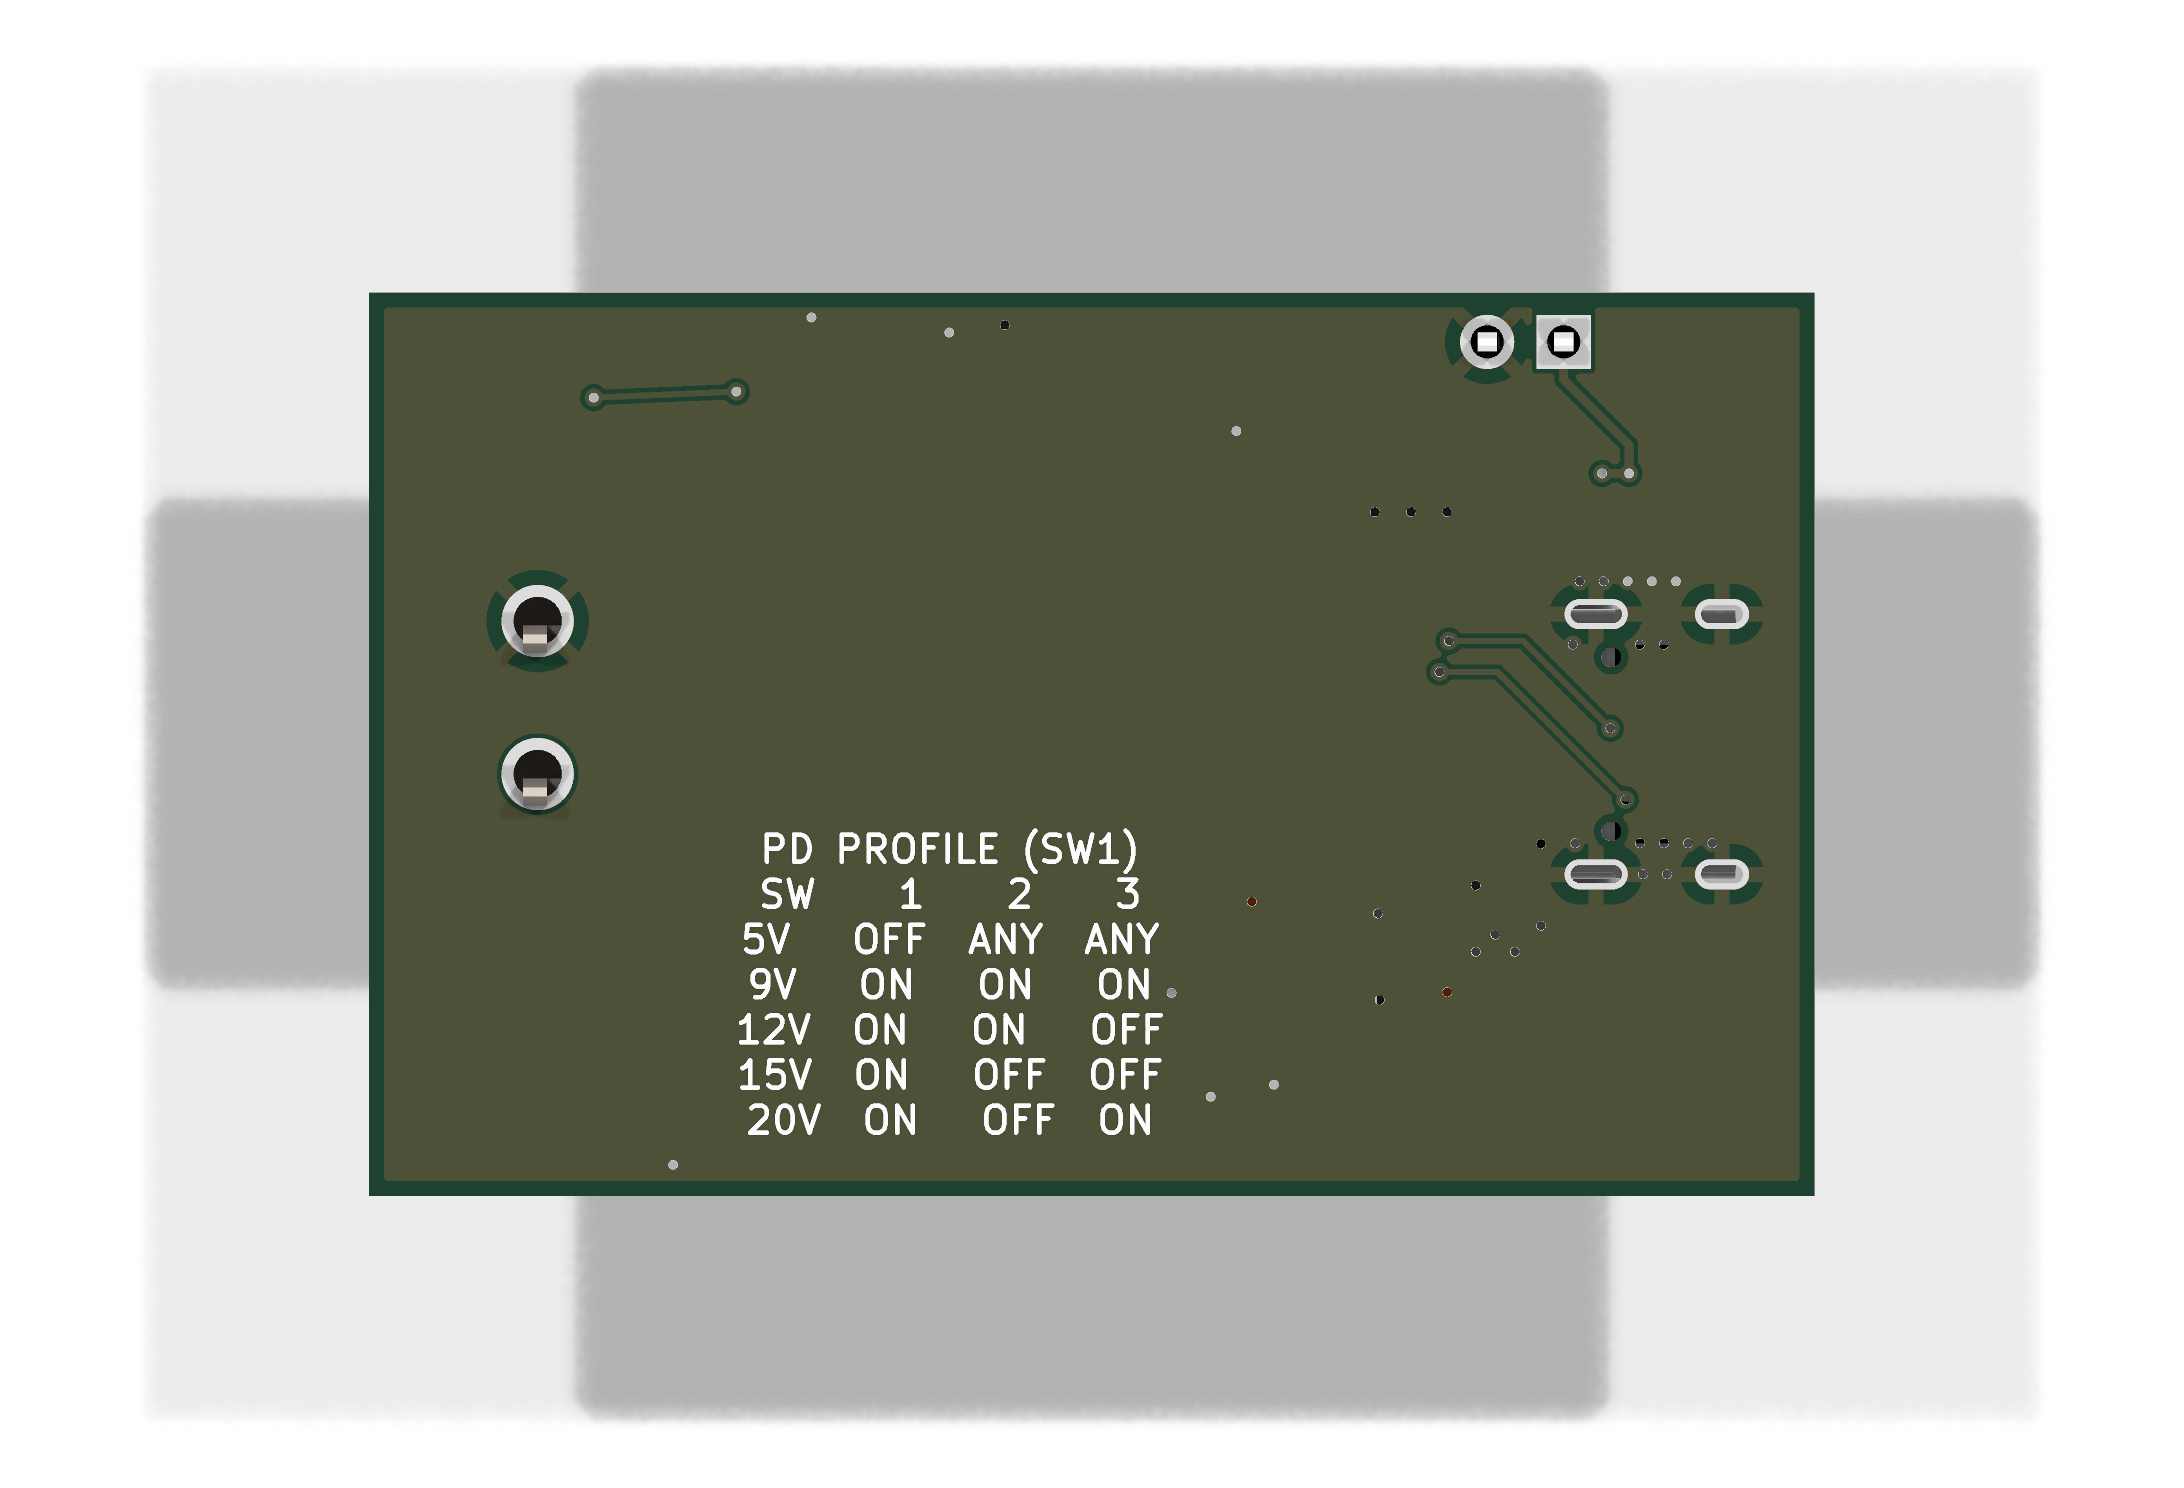
\includegraphics[width=0.48\textwidth]{bottom.png}
\caption{Assembled-view renders. Left: top --- USB-C at left, 5\,A corridor
to the screw terminal at right, DIP selector top edge, LED row bottom.
Right: bottom --- ground pour and the mirrored profile table.}
\end{figure}

\begin{figure}[h]\centering
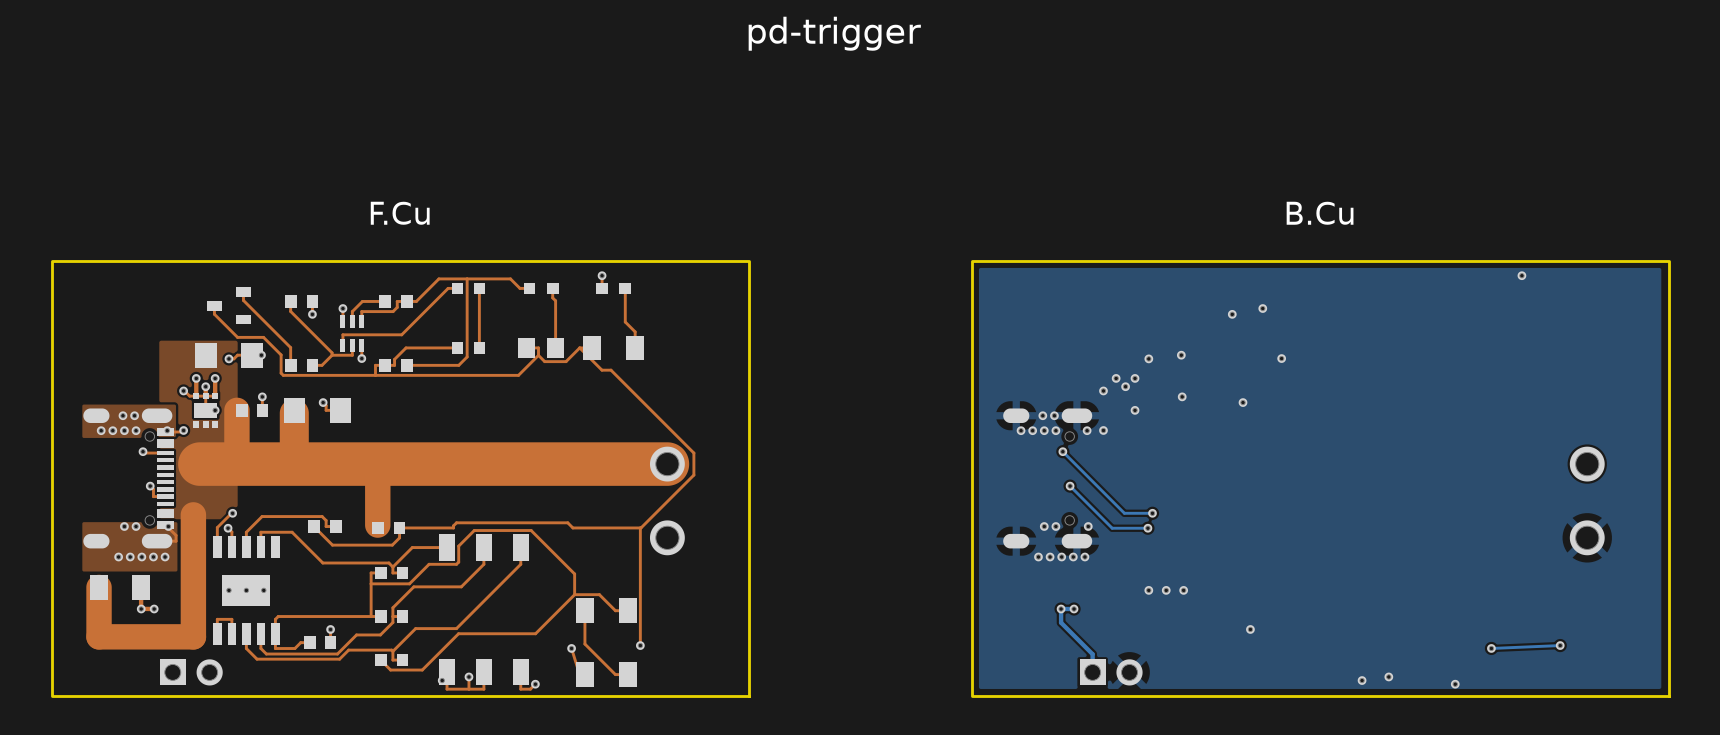
\includegraphics[width=\textwidth]{pd-trigger_layers.png}
\caption{Copper layers from the fabrication gerbers. F.Cu: pour fan-in at
J1, 3\,mm trunk, ground lobes. B.Cu: return pour, ground stitching.}
\end{figure}

\clearpage
\section{Verification record}
\begin{center}
\begin{tabular}{@{}llll@{}}
\toprule
Gate & Phase & Criterion & Result\\
\midrule
erc & P4 & errors + warnings $=0$ & \textbf{pass} 0/0\\
place & P6 & legality, edges, decouplers & \textbf{pass} 0/0\\
drc\_routed & P7 & parity + all track checks, err+warn $=0$ & \textbf{pass} 0/0\\
verify & P8 & 8-check suite, error severity $=0$ & \textbf{pass} 8/8\\
dfm & P9 & gerber-side DFM, error severity $=0$ & \textbf{pass} 0 err\\
\bottomrule
\end{tabular}
\end{center}

Two independent adversarial reviews (schematic, board) ran with fresh
context. Notable outcomes: the schematic review verified the window
truth table at 4.4/5.25/6.7/9/20\,V and the transistor pin map against the
manufacturer table; the board review caught (and the pipeline fixed) an
initially undersized ground-return attachment at J1 and the then-missing
functional silk package.

\subsection{Standing waivers}
\begin{itemize}\itemsep2pt
  \item \textbf{W1} DP/DM short-at-chip: accepted as hardware-safer;
  PD-only capability is the documented cost.
  \item \textbf{W2} CH224K quiescent current unpublished: bounded by
  arithmetic (0.979\,mA worst corner vs.\ 1.7\,mA budget) and by WCH's own
  reference circuit; measured at bring-up.
  \item C1B bulk-cap feed crosses the pour through 1.11+1.25\,mm channels
  (checker-blind geometry, disclosed): dead-end stub, $\sim$0.3\,A ripple
  vs.\ 3.49\,A capacity.
  \item J1 mouth sits $\sim$0.5\,mm inboard of the board edge; thick
  cable overmolds may not latch --- respin note.
\end{itemize}

\section{Bill of materials}
24 lines, 28 placed references. Ext.\ = JLC Extended (feeder fee applies).
Prices are qty-1 LCSC references.

{\small
\begin{longtable}{@{}p{4.2cm}p{4.2cm}p{2.6cm}lll@{}}
\toprule
MPN & Value / description & Package & LCSC & Tier & \$\\
\midrule
\endhead
CH224K &  & ESSOP-10-150mil-1mm & C970725 & Ext. & 0.389 \\
USB4105-GF-A-120 & USB-C receptacle 16P SMT & SMD & C5184243 & Ext. & 0.9247 \\
KF128-5.08-2P-AA & Screw terminal 5.08mm 2P & Plugin,P=5.08mm & C474952 & Ext. & 0.19 \\
HX PZ2.54-1x2P ZZ & 1x2 2.54mm male THT & Plugin,P=2.54mm & C32713268 & Ext. & 0.0158 \\
TVS2200DRVR & 22V flat-clamp TVS, unidirectional & WSON-6-EP(2x2) & C523793 & Ext. & 0.3777 \\
BZX84C6V2 & 6.2V zener & SOT-23 & C841160 & Ext. & 0.0196 \\
XL-1608SYGC-06 & Yellow-green LED 0603, Vf 2.2V & 0603 & C965805 & Ext. & 0.0074 \\
F.0603.00011/P2-0603R4TS2-06T-001 & Red LED 0603, Vf 2.2V, 100mcd@5mA & 0603 & C7496813 & Ext. & 0.0108 \\
BC847BS & Dual NPN, SOT-363 & SOT-363 & C41375126 & Ext. & 0.0283 \\
2.54-3P TPGT & 3-position SPST DIP switch, SMD 2. & SMD,P=2.54mm & C7421520 & Ext. & 0.4083 \\
BSMD1206-100-30V & PPTC 1.0A hold / 1.8A trip, 30V, 1 & 1206 & C5358568 & Ext. & 0.0988 \\
CL31A106KBHNNNE & 10uF 50V X5R (2x, forms the C1 22u & 1206 & C13585 & Basic & 0.3735 \\
CC0603KRX7R9BB104 & 100nF 50V X7R & 0603 & C14663 & Basic & 0.0241 \\
CL10A105KB8NNNC & 1uF 50V X5R & 0603 & C15849 & Basic & 0.0966 \\
0603WAF1002T5E & 10k & 0603 & C25804 & Basic & 0.0077 \\
0603WAF1003T5E & 100k & 0603 & C25803 & Basic & 0.0079 \\
1206W4J0511T5E & 510R (x2 in series, \textasciitilde{}1k dropper) & 1206 & C25386 & Ext. & 0.0112 \\
0603WAF6801T5E & 6.8k & 0603 & C23212 & Basic & 0.0029 \\
0603WAF4701T5E & 4.7k & 0603 & C23162 & Basic & 0.0117 \\
0603WAF4702T5E & 47k & 0603 & C25819 & Basic & 0.0112 \\
RC1206FR-073K3L & 3.3k & 1206 & C137292 & Ext. & 0.0178 \\
0603WAF1501T5E & 1.5k & 0603 & C22843 & Basic & 0.0023 \\
0805W8F4701T5E & 4.7k & 0805 & C17673 & Basic & 0.011 \\
0603WAF0000T5E & 0R & 0603 & C21189 & Basic & 0.0027 \\
\bottomrule
\end{longtable}
}

\section{Ordering and bring-up}
Estimated \$19.65 for 10 assembled (\$1.96/board; the JLC cart is the only
real quote). Human steps before ordering, from \texttt{fab/order.json}:
\begin{enumerate}\itemsep2pt
  \item \textbf{Select 2\,oz copper} on the JLC order page (the 5\,A path
  depends on it; the default is 1\,oz).
  \item Upload the gerber zip to jlcdfm.com and the quote page; review
  their DFM report.
  \item In the assembly preview, check every polarized part's rendered
  orientation (LEDs, zener, TVS, tantalum-free board --- diode-class parts).
  \item Hand-solder \net{J2}/\net{J3} through-hole parts after SMT delivery.
  \item Bring-up: measure \net{/VDD} at the 5\,V profile (W2); buzz out
  \net{Q1} E/B/C once; continuity-check \net{SW1} pins 1--3 unpressed;
  use an e-marked cable and a genuine PD source for any $>$3\,A draw.
\end{enumerate}

\vfill
\begin{center}\footnotesize\color{gray}
Generated by the ai-ee v1 pipeline (workspace \texttt{boards/pd-trigger},
S14 run~c). Sources: requirements.md, architecture/, reports/, fab/order.json.
\end{center}
\end{document}
